%=====================================================================
%  MANUSCRIPT v2 — IEEE journal style (IEEEtran)
%  Hybrid Ant-Colony Metaheuristics for QoS-Aware Traffic-Engineering
%  Optimization in Software-Defined Networks: Formulation, Exact
%  Certification, Statistical Evaluation, and SRv6 Mapping
%
%  Compile: pdflatex -> pdflatex (bibtex-free, manual bibliography)
%  Numbers are injected from results/macros.tex and results/tables/*.tex
%  produced by experiments/exp6_tables.py (fully reproducible pipeline).
%=====================================================================
\documentclass[journal]{IEEEtran}
\usepackage{cite}
\usepackage{amsmath,amssymb,amsfonts}
\usepackage{graphicx}
\usepackage{textcomp}
\usepackage{booktabs}
\usepackage{url}
\newcommand{\FO}{\mathrm{FO}}
\newcommand{\PoolOptFO}{132}
\newcommand{\GaFOmaia}{132.0}
\newcommand{\GaFOmaiaCI}{0.0}
\newcommand{\DeFOmaia}{132.0}
\newcommand{\DeFOmaiaCI}{0.0}
\newcommand{\QlFOmaia}{130.2}
\newcommand{\QlFOmaiaCI}{0.8}
\newcommand{\DjFOmaia}{120}
\newcommand{\DjMaxUtil}{2.10}
\newcommand{\CspfFOmaia}{132}
\newcommand{\CspfMaxUtil}{1.00}
\newcommand{\IlpZmaia}{0.872}
\newcommand{\IlpZmaiaHigh}{0.984}
\newcommand{\IlpZmaiaHighPct}{98.4}
\newcommand{\IlpZmaiaMax}{0.984}
\newcommand{\IlpZWaxMax}{0.872}
\newcommand{\IlpZGridMax}{0.872}
\newcommand{\IlpInfeasLoad}{>1.5}
\newcommand{\IlpInfeasGrid}{--}
\newcommand{\IlpTime}{0.3}
\newcommand{\PoolTime}{0.1}
\newcommand{\LoadRatioHigh}{1.13}
\newcommand{\LoadRatioMax}{1.26}
\newcommand{\QlFeasNominal}{40}
\newcommand{\AntDjMaxUtil}{1.70}
\newcommand{\AntDjViol}{2}
\newcommand{\AntDjFO}{128}
\newcommand{\AntCspfMaxUtil}{1.52}
\newcommand{\AntCspfViol}{1}
\newcommand{\AntCspfFO}{130}
\newcommand{\AntGaFeas}{85}
\newcommand{\AntGaFO}{131.7$\pm$0.3}
\newcommand{\AntDeFeas}{10}
\newcommand{\AntDeFO}{130.2$\pm$0.3}
\newcommand{\AntQlFeas}{0}
\newcommand{\AntQlFO}{129.8$\pm$0.3}
\newcommand{\AntPoolOpt}{132}
\newcommand{\AntPoolOptFeasRate}{95}
\newcommand{\GerZ}{0.870}
\newcommand{\GeantZ}{0.870}
\newcommand{\GaFeasAllInst}{94}
\newcommand{\AntDelayGerMin}{1.0}
\newcommand{\AntDelayGerMax}{1.8}
\newcommand{\AntDelayGerMean}{1.1}
\newcommand{\AntCapGer}{2.00}
\newcommand{\AntDelayGeantMin}{1.0}
\newcommand{\AntDelayGeantMax}{16.6}
\newcommand{\AntDelayGeantMean}{4.6}
\newcommand{\AntCapGeant}{2.89}
\newcommand{\GaViolHigh}{0.0}
\newcommand{\GaViolHighCI}{0.0}
\newcommand{\DeViolHigh}{0.2}
\newcommand{\DeViolHighCI}{0.2}
\newcommand{\QlViolHigh}{1.8}
\newcommand{\QlViolHighCI}{0.7}
\newcommand{\CspfViolHigh}{0.0}
\newcommand{\CspfViolHighCI}{0.0}
\newcommand{\DjViolHigh}{6.0}
\newcommand{\DjViolHighCI}{0.0}
\newcommand{\GaViolMax}{1.1}
\newcommand{\GaViolMaxCI}{0.4}
\newcommand{\DeViolMax}{1.9}
\newcommand{\DeViolMaxCI}{0.4}
\newcommand{\QlViolMax}{1.9}
\newcommand{\QlViolMaxCI}{0.5}
\newcommand{\CspfViolMax}{4.0}
\newcommand{\CspfViolMaxCI}{0.0}
\newcommand{\DjViolMax}{9.0}
\newcommand{\DjViolMaxCI}{0.0}
\newcommand{\GaFeasMaiaNominal}{100}
\newcommand{\GaFeasMaiaHigh}{100}
\newcommand{\GaFeasMaiaMax}{20}
\newcommand{\GaFeasGeantNominal}{85}
\newcommand{\GaFeasGeantHigh}{90}
\newcommand{\GaFeasGeantMax}{55}
\newcommand{\GaViolGeantNominal}{0.1$\pm$0.2}
\newcommand{\QlVsGaP}{<0.001}
\newcommand{\GaTime}{6.4}
\newcommand{\DeTime}{5.1}
\newcommand{\QlTime}{1.1}
\newcommand{\SrvOfMaia}{69}
\newcommand{\SrvRedMaia}{4.1}
\newcommand{\MaxSLMaia}{6}
\newcommand{\SrhMaia}{144}
\newcommand{\SrvOfWax}{35}
\newcommand{\SrvRedWax}{2.1}
\newcommand{\MaxSLWax}{4}
\newcommand{\SrhWax}{112}
\newcommand{\SrvOfGrid}{70}
\newcommand{\SrvRedGrid}{4.1}
\newcommand{\MaxSLGrid}{10}
\newcommand{\SrhGrid}{208}
\newcommand{\SrvOfGer}{51}
\newcommand{\SrvRedGer}{3.0}
\newcommand{\MaxSLGer}{6}
\newcommand{\SrhGer}{144}
\newcommand{\SrvOfGeant}{39}
\newcommand{\SrvRedGeant}{2.3}
\newcommand{\MaxSLGeant}{8}
\newcommand{\SrhGeant}{176}
\newcommand{\SrvSrRules}{17}
\newcommand{\MaxSLAll}{10}
\newcommand{\MaxSrhBytes}{208}
\newcommand{\MeanSLWax}{3.1}
\newcommand{\UrllcDoptOne}{52}
\newcommand{\UrllcDdjOne}{265}
\newcommand{\UrllcDoptTwo}{163}
\newcommand{\UrllcDdjTwo}{212}
\newcommand{\UrllcDoptThree}{233}
\newcommand{\UrllcDoptFifteen}{91}
\newcommand{\UrllcLossOptFifteen}{3.3}
\newcommand{\UrllcLoptOne}{0.0}
\newcommand{\UrllcLossOptTwo}{4.7}
\newcommand{\UrllcLdjOne}{53.1}
\newcommand{\UrllcLossDjTwo}{72.5}
\newcommand{\UrllcLossDjFour}{78.9}
\newcommand{\GerDoptOne}{16}
\newcommand{\GerDdjOne}{147}
\newcommand{\GerDoptTwo}{29}
\newcommand{\GerDdjTwo}{182}
\newcommand{\GerDoptThree}{72}
\newcommand{\GerDoptFifteen}{16}
\newcommand{\GerLossOptFifteen}{0.0}
\newcommand{\GerLoptOne}{0.0}
\newcommand{\GerLossOptTwo}{0.0}
\newcommand{\GerLdjOne}{14.6}
\newcommand{\GerLossDjTwo}{2.8}
\newcommand{\GerLossDjFour}{4.4}
\newcommand{\NumSimSeeds}{5}
\newcommand{\SimDelayOpt}{63}
\newcommand{\SimDelayDj}{220}
\newcommand{\SimJitOpt}{1.2}
\newcommand{\SimJitDj}{1.6}
\newcommand{\SimLossOpt}{0.0}
\newcommand{\SimLossDj}{26.7}
\newcommand{\SimThrGain}{+38\%}
\newcommand{\SimDelayRatio}{3.5}
\newcommand{\SimLossRatio}{--}
\newcommand{\TotalDemand}{9.70}


\begin{document}

\title{Hybrid Ant-Colony Metaheuristics for QoS-Aware Traffic-Engineering
Optimization in Software-Defined Networks: Formulation, Exact Certification,
Statistical Evaluation, and SRv6 Mapping}
\author{João~Paulo~Versiani~Ladeia,~and~Nilton~Alves~Maia%
\thanks{Manuscript received XXX; revised XXX. The authors are with the
Graduate Program in Computational Modeling and Systems (PPGMCS),
Universidade Estadual de Montes Claros, Montes Claros, Brazil.}}

\markboth{Software-Defined Networking Traffic Engineering}{Ladeia \& Maia}

\maketitle

\begin{abstract}
The growth of Internet traffic makes capacity expansion a recurring capital
expense and motivates traffic engineering (TE) as a software-based
alternative. Software-Defined Networking (SDN) exposes the routing layer to
programmatic control, enabling QoS-aware path computation. This paper
formulates simultaneous routing of heterogeneous application flows as a
constrained combinatorial optimization problem and solves it with a two-stage
hybrid: an Ant Colony Optimization stage (AntNet) builds a pool of loop-free
candidate routes, and a Genetic Algorithm (ACO$+$GA) or Differential Evolution
(ACO$+$DE) selects the route set. Beyond the original scoring function, we
introduce a revised formulation in which capacity and end-to-end delay are
\emph{hard} constraints and load balancing is an explicit min--max link
utilization objective, and we solve it exactly as a binary multi-commodity
flow (ILP). On a 52-node network and two synthetic 52-node topologies, over
five load factors and twenty randomized replications, the exact ILP
certifies that the pool-augmented hybrid attains the optimum of its search
space in every replication and, more importantly, computes \emph{exact
bottleneck lower bounds} --- proving, e.g., that at $1.25\times$ load on the
sparse instance no routing can keep every link below \IlpZmaiaHighPct\%
utilization, where shortest-path routing reaches \DjMaxUtil$\times$
capacity and inflicts \DjViolHigh\ SLA violations against zero for the
hybrid. Packet-level simulation shows
the optimized network sustaining URLLC-grade flows within a 150\,ms delay
budget up to $2\times$ background amplification, whereas shortest-path
routing violates the same budget at every tested load. A measured data-plane
study shows that mapping the optimized paths to SRv6 segment lists reduces
forwarding state by \SrvRedMaia$\times$ (from \SrvOfMaia\ per-flow OpenFlow
rules to \SrvSrRules\ headend rules) relative to per-flow OpenFlow
programming. The results position deterministic, constraint-explic\-it
metaheuristics --- with exact certification --- as a practical and auditable
traffic-engineering core for SDN controllers, and delimit precisely when
they are preferable to learning-based routing.
\end{abstract}

\begin{IEEEkeywords}
Software-defined networking, traffic engineering, QoS routing, ant colony
optimization, genetic algorithm, differential evolution, exact optimization,
SRv6, network slicing, deep reinforcement learning.
\end{IEEEkeywords}

%=====================================================================
\section{Introduction}
\IEEEPARstart{O}{perators} face a structural tension: traffic grows faster
than revenue, and capacity expansion is a recurring capital expense.
Traffic engineering (TE) attacks this tension from the software side --- it
routes the traffic that exists more intelligently instead of adding links.
Software-Defined Networking (SDN) supplies the missing control point: by
decoupling the control plane and exposing programmable forwarding
\cite{mckeown2008,kim2013,hu2014}, an SDN controller can compute and install
paths that satisfy per-application requirements instead of replicating
shortest-path behavior.

This paper studies exactly that problem: given a topology with per-link
capacity and delay, and a set of $L$ concurrent applications with minimum
bandwidth, maximum delay and priority requirements, compute a route for
every application that maximizes admission quality under QoS constraints.
We make the following contributions, each of which responds to a concrete
methodological gap in the literature on heuristic SDN-TE:
\begin{enumerate}
\item \textbf{Revised formulation.} We analyze the scoring-function model
commonly used in heuristic SDN-TE, identify its degeneracies (constant terms
under full admission; capacity counted against a flow cardinality), and
reformulate the problem with \emph{hard} capacity and delay constraints and
an explicit min--max utilization balancing objective
(Section~\ref{sec:model}).
\item \textbf{Exact certification.} We solve the revised model exactly as a
binary multi-commodity flow ILP and the scoring model exactly over the
candidate pool. The exact solutions (i) certify that the pool-augmented
hybrid attains the pool optimum in every replication, and (ii) compute
\emph{exact bottleneck lower bounds} --- proofs of the minimum achievable
maximum link utilization --- a property no heuristic can claim, which
exposes how far greedy and learning-based baselines sit from the provable
optimum (Section~\ref{sec:cert}).
\item \textbf{Statistical evaluation at scale.} We evaluate six routing
methods on three topologies across five load factors and twenty randomized
replications, with 95\% confidence intervals and Wilcoxon signed-rank tests,
identifying the load regime in which the hybrid strictly dominates greedy
and learning-based baselines (Section~\ref{sec:sweep}).
\item \textbf{Measured SRv6 state reduction.} We map the optimized paths to
SRv6 segment lists \cite{rfc8402,rfc8754,rfc8986} and \emph{measure} the
data-plane state on all topologies, quantifying the reduction with respect
to per-flow OpenFlow rules and bounding the SRH overhead
(Section~\ref{sec:srv6}).
\item \textbf{Slice isolation evidence.} We connect the demand profile to
3GPP service classes \cite{itu-m2083,3gpp-ts23501} and measure, in
packet-level simulation, the stability of URLLC-grade flows under growing
background load --- comparing optimized against shortest-path routing
(Section~\ref{sec:slices}).
\item \textbf{Learning-based baseline.} We implement a tabular Q-learning
routing agent with the same state--action structure as DRL routers and
benchmark it under the same protocol, grounding the DRL discussion in
measured numbers rather than assertions (Section~\ref{sec:qlb}).
\end{enumerate}

The remainder is organized as follows.
Section~\ref{sec:related} reviews related work.
Section~\ref{sec:model} presents the system model.
Section~\ref{sec:method} describes the algorithms.
Sections~\ref{sec:srv6} and~\ref{sec:slices} present the SRv6 mapping and
slice differentiation.
Section~\ref{sec:setup} details the experimental methodology,
Section~\ref{sec:results} reports results, Section~\ref{sec:limits} discusses
threats to validity, and Section~\ref{sec:conc} concludes.

%=====================================================================
\section{Related Work}
\label{sec:related}
\textbf{Heuristic and hybrid routing.} Ant-based routing originates with
AntNet \cite{dorigo2004}, and ACO has been applied to QoS routing
repeatedly since. Two-stage ``generate-and-select'' hybrids --- a constructive
stage feeding an evolutionary selector --- are the standard memetic pattern;
the present work instantiates it for SDN with an explicit admission-scoring
objective and, critically, adds exact certification that prior hybrid-routing
studies omit.

\textbf{Learning-based routing.} DRL for SDN routing has progressed from
experience-driven proposals \cite{xu2018experience,stampa2017drl} to
evaluated traffic-engineering agents \cite{almasan2022drl}. Reported
strengths are online adaptivity and traffic-matrix generalization; reported
costs are large training campaigns and the sim-to-real gap. Our experiments
(Section~\ref{sec:qlb}) add a controlled, constraint-explicit comparison on
identical instances.

\textbf{Programmable data planes.} OpenFlow \cite{mckeown2008} programs
switches with per-flow rules; P4 \cite{bosshart2014} generalizes parsing and
matching. Both expose the TCAM-pressure problem that motivates SRv6
\cite{rfc8402,rfc8754,rfc8986,rfc9256}: the path state is carried in the
packet, and only headends hold policy state. To our knowledge, the state
reduction of routing-optimizer output under SRv6 has not been measured on
fixed topologies with optimizer-produced paths; Section~\ref{sec:srv6}
reports it.

\textbf{Network slicing.} 3GPP defines slice/service types and QoS flows
\cite{3gpp-ts23501} anchored on the IMT-2020 usage scenarios
\cite{itu-m2083}. Transport-side slice isolation is usually pursued with
dedicated resources; we show that constraint-explicit routing yields
measurable logical isolation without physical partitioning
(Section~\ref{sec:slices}).

%=====================================================================
\section{System Model and Problem Formulation}
\label{sec:model}
The network is a directed graph $G=(V,E)$, $|V|=n$; link $(i,j)\in E$ has
capacity $\mu_{ij}$ (Mbps) and one-way delay $c_{ij}$ (ms). A set of $L=17$
applications must be routed concurrently; application $k$ requires nominal
flow $\lambda_k$ (Mbps), tolerates end-to-end delay $h_k$ (ms) and carries
priority $\delta_k$. Let $x_{ij}^{k}\in\{0,1\}$ indicate whether the route of
application $k$ uses link $(i,j)$.

\subsection{Original Scoring Model}
\label{sec:origfo}
The original model maximizes the weighted admission score
\begin{equation}
\FO \;=\; \sum_{k=1}^{L}\delta_k\,y_k
   + p_1\sum_{k=1}^{L} y_k
   + p_2\sum_{k=1}^{L} w_k
   + p_3\sum_{k=1}^{L} t_k,
\label{eq:fo}
\end{equation}
with $p_1{=}3$, $p_2{=}2$, $p_3{=}1$; $y_k$ marks an established connection,
$w_k$ capacity-sufficient routes and $t_k$ delay-conforming routes. Two
structural observations motivate the revised model: (i) under full admission
every $y_k=1$, so the first two sums are constant and the score reduces to
$\FO = \Sigma\delta_k + 4L - 2\,n_{\mathrm{over}} - n_{\mathrm{dv}}$, where
$n_{\mathrm{over}}$ counts overloaded \emph{links} and $n_{\mathrm{dv}}$
counts delay-violating \emph{flows}; (ii) the mixed cardinality (links vs.\
flows) makes weights comparable only by accident. The score saturates at
$\FO^{*}=\Sigma\delta_k+4L$: any fully feasible solution attains it, and the
score cannot discriminate among solutions with different load balance.

\subsection{Revised Model: Hard Constraints and Balancing}
\label{sec:revfo}
We therefore evaluate solutions on a revised model that separates
feasibility from quality:
\begin{align}
\text{capacity (hard):}\quad
&\sum_{k=1}^{L}\lambda_k\,x_{ij}^{k} \;\le\; \mu_{ij}
\qquad \forall (i,j)\in E, \label{eq:hardcap}\\
\text{delay (hard):}\quad
&\sum_{(i,j)\in E} c_{ij}\,x_{ij}^{k} \;\le\; h_k
\qquad \forall k, \label{eq:harddel}\\
\text{balance (objective):}\quad
&\min\; Z,\ \ Z \;\ge\;
\frac{1}{\mu_{ij}}\sum_{k=1}^{L}\lambda_k\,x_{ij}^{k}
\quad \forall (i,j). \label{eq:minmax}
\end{align}
A solution is \emph{feasible} iff \eqref{eq:hardcap} and \eqref{eq:harddel}
hold for all links and flows; among feasible solutions we prefer minimum
maximum utilization $Z$. When \eqref{eq:hardcap}--\eqref{eq:harddel} admit no
solution at all (certified by the exact model), every heuristic output
violates some constraint, and the natural metric becomes the number of
violations it inflicts.

%=====================================================================
\section{Routing and Optimization Methods}
\label{sec:method}

\subsection{Stage 1: Candidate-Route Generation (ACO/AntNet)}
For each application an ant colony builds source--destination walks with the
transition probability
\begin{equation}
P(i,j)=\frac{[\tau_{ij}]^{\alpha}[\eta_{ij}]^{\beta}}
{\sum_{l\in\mathcal{N}_i}[\tau_{il}]^{\alpha}[\eta_{il}]^{\beta}},
\label{eq:aco}
\end{equation}
repeated nodes are removed, links reinforce pheromone proportionally to the
carried bandwidth, and evaporation rate $\rho$ maintains diversity. With
$100$ ants $\times$ $100$ iterations this yields 362--1014 distinct candidate
routes per topology (Table~\ref{tab:topo}).

\subsection{Stage 2: Route-Set Selection (ACO$+$GA / ACO$+$DE)}
An individual is an integer vector selecting one pool route per application
(each selection constrained to its application's block). The GA applies
roulette selection (pressure 8), arithmetic crossover ($\gamma{=}0.4$) and
Gaussian mutation; DE applies rand/1 mutation
($\beta\sim\mathcal{U}(0.2,0.8)$) with binomial crossover ($p_{CR}{=}0.2$).
Both maximize \eqref{eq:fo} with $300$ generations over $50$ individuals.
\emph{Pool augmentation.} Two constructive augmentations make the selector's
search space self-sufficient: (i) for load factors $f>1$, each additional
background flow receives $k$-shortest-delay candidate paths; (ii) for every
flow, the CSPF constructive route is inserted into its block. Augmentation
(ii) guarantees that the selector's optimum is never worse than CSPF --- the
CSPF assembly is inside the search space --- while remaining free to improve
on it whenever the pool holds a better combination. This closes the
classical objection against generate-and-select designs: pool diversity, not
the selector, becomes the binding constraint, and the augmentation pins the
selector to at least the constructive baseline.

\subsection{Baselines}
\textbf{Dijkstra.} Each application follows the Euclidean-shortest path ---
the behavior implicitly replicated by shortest-path IGP routing.
\textbf{CSPF.} Constrained shortest path first: flows are admitted in
priority order; links whose residual capacity is below the request are
pruned; the delay-minimizing path on the pruned graph is selected; if no
pruned path satisfies the delay budget the flow is admitted on an
unconstrained path (honest best-effort, counted as a violation when it
overloads links).
\textbf{Q-learning.} A tabular, per-flow, sequential learning agent with
node-state/neighbor-action structure, $\epsilon$-greedy exploration,
capacity-penalty shaping, and a capacity-pruned greedy rollout
(Section~\ref{sec:qlb}).
\textbf{ILP (exact).} Two exact formulations close the methodological loop:
(i) \emph{ILP-P} maximizes \eqref{eq:fo} over the same pool explored by the
GA/DE, certifying the metaheuristics' optimality gap; (ii) \emph{ILP-L}
solves the revised model \eqref{eq:hardcap}--\eqref{eq:minmax} exactly as a
binary multi-commodity flow with min--max utilization, certifying
feasibility or infeasibility of each instance.

%=====================================================================
\section{SRv6 Data-Plane Mapping and Measured State Reduction}
\label{sec:srv6}
Per-flow OpenFlow programming stores one match--action rule per flow at
every transit switch; the aggregate state is
$\Phi_{\mathrm{OF}}=\sum_{k}(|p_k|-1)\le K L_{\max}$
\cite{mckeown2008}. SRv6 \cite{rfc8402,rfc8754,rfc8986} carries the path
state in the packet: each node $v$ is assigned a Segment Identifier
$\sigma(v)=\mathrm{LOC}(v){:}{:}\mathrm{FUNC}_{\mathrm{End}}$
\cite{rfc8986}, and the optimal route
$p^{*}_k=(v^{(k)}_1,\ldots,v^{(k)}_{m_k})$ is encoded as the segment list
\begin{equation}
\mathcal{SL}_k=\mathrm{rev}\bigl[\sigma(v^{(k)}_2),\ldots,
\sigma(v^{(k)}_{m_k})\bigr],
\label{eq:seglist}
\end{equation}
so that on arrival at $v^{(k)}_i$ the outer destination equals
$\sigma(v^{(k)}_i)$ and $\mathrm{SegmentsLeft}=m_k-i$; the flow-agnostic
\texttt{End} function advances the segment and the egress decapsulates.
Because the ACO stage removes repeated nodes, $p^{*}_k$ is a simple path and
the SRH is well formed (no micro-loops). The two-stage optimizer thereby acts
as a centralized Path Computation Element \cite{rfc4655}: it emits for each
flow a Segment Routing Policy $\Pi_k=\langle H_k, C_k, \mathcal{SL}_k\rangle$
\cite{rfc9256} whose color $C_k$ carries the serving slice identifier; the
controller programs only headends.

Under this mapping the per-node rule footprint is
\begin{equation}
\Phi_{\mathrm{SR}}(v)=\begin{cases}
|\{k: v=v^{(k)}_1\}| & \text{if $v$ is a headend},\\
0 & \text{otherwise},
\end{cases}
\label{eq:srstate}
\end{equation}
i.e., $\mathcal{O}(K)$ globally and $\mathcal{O}(1)$ per transit node.
Section~\ref{sec:srv6res} reports the \emph{measured} counts on all three
topologies together with the SRH encapsulation overhead
($40+8+16\,|\mathcal{SL}_k|$ bytes per packet).

%=====================================================================
\section{5G/6G Slice Differentiation and SLA Guarantees}
\label{sec:slices}
The 17 applications instantiate the three IMT-2020 service classes
\cite{itu-m2083} with the standardized slice/service types of 3GPP TS
23.501 \cite{3gpp-ts23501}: \emph{URLLC} (SST $=2$) gathers conversational
voice and interactive control (apps 8, 9, 13, 15; $h_k=150$\,ms, maximal
priority $\delta_k=5$); \emph{eMBB} (SST $=1$) gathers high-definition video
(apps 3, 4, 11, 12; $1.20$--$1.74$\,Mbps); \emph{mMTC} (SST $=3$) gathers
telemetry and elastic transfer (apps 1, 2, 5, 6, 7, 10, 14, 16, 17;
$h_k=1000$\,ms). Isolation follows from the constraint structure: the
capacity constraint \eqref{eq:hardcap} is evaluated on the \emph{aggregate}
cross-slice offered load of each link, so a feasible solution structurally
prevents one slice from congesting another; the priority term of
\eqref{eq:fo} biases admission toward URLLC; and the delay constraint binds
each route to its slice budget. The result is deterministic, priority-ordered
degradation instead of cross-slice interference, obtained without physical
sharding. Section~\ref{sec:slicesres} measures this directly: URLLC-grade
flows keep their 150\,ms budget under growing background amplification with
optimized routing, and do not under shortest-path routing.

%=====================================================================
\section{Experimental Methodology}
\label{sec:setup}
\subsection{Topologies and Demands}
We evaluate three 52-node instances (Fig.~\ref{fig:topos}):
\emph{maia52} --- the original study topology (66 links, uniform 2\,Mbps,
delays 1--80\,ms); \emph{waxman52} --- a connected Waxman random graph
\cite{waxman1988} (177 links, geometric delays); \emph{gridcore} --- a
48-node peripheral grid plus a 4-node dense core (96 links, 1\,ms
peripheral / 20\,ms core delays). The 17-flow demand profile of
Table~\ref{tab:apps} (total \TotalDemand\,Mbps) is applied to all
instances, with endpoints re-drawn on the synthetic graphs and connectivity
guaranteed.

\begin{table}[!t]
\caption{Application demands (all topologies): nominal flow, delay budget
and priority. Classes per Section~\ref{sec:slices}.}
\label{tab:apps}
\centering
\begin{tabular}{@{}llrrr@{}}
\toprule
Class & Apps & $\lambda_k$ (Mbps) & $h_k$ (ms) & $\delta_k$\\
\midrule
URLLC & 8, 9, 13, 15 & 0.512 & 150 & 5\\
eMBB  & 3, 4, 11, 12  & 1.20--1.74 & 150 & 0--5\\
mMTC  & 1, 2, 5, 6, 7, 10, 14, 16, 17 & 0.256 & 1000 & 0\\
\bottomrule
\end{tabular}
\end{table}

\begin{table}[!t]
\caption{Topology instances and ACO candidate-pool sizes (100 ants
$\times$ 100 iterations, 20 seeds).}
\label{tab:topo}
\centering
\begin{tabular}{@{}lrrrl@{}}
\toprule
Instance & Nodes & Links & Mean deg. & Pool size (routes)\\
\midrule
maia52 & 52 & 66 & 2.54 & 362--420\\
waxman52 & 52 & 177 & 6.81 & 927--1014\\
gridcore & 52 & 96 & 3.69 & 706--780\\
\bottomrule
\end{tabular}
\end{table}

\subsection{Load Sweep and Replication}
For $f\le 1$ all flow demands are scaled by the load factor
$f\in\{0.5, 0.75, 1.0\}$; for $f>1$ (loads $\{1.25, 1.5\}$) the nominal
flows are kept at nominal rate and
$\mathrm{round}((f{-}1)\!\cdot\!20)$ additional concurrent background data
flows ($0.256$\,Mbps, $h_k{=}1000$\,ms) are added on random connected
endpoint pairs --- modeling network growth as new sessions rather than
inflating existing flows beyond the physical link capacity, which would
certify infeasibility trivially. Stochastic methods (ACO$+$GA,
ACO$+$DE, Q-learning) are replicated over $20$ seeds per (topology, load);
the ACO candidate pool is generated once per (topology, seed) at nominal
load and reused across the sweep, since pool diversity is a property of the
topology rather than of the load; route selection adapts to load.
Deterministic methods (Dijkstra, CSPF, ILP) run once per (topology, load).
All experiments use fixed seeds and are fully reproducible from the released
scripts.

\subsection{Metrics and Statistics}
For every solution we record: the original score \eqref{eq:fo}; feasibility
under \eqref{eq:hardcap}--\eqref{eq:harddel}; maximum link utilization $Z$;
the number of capacity-violating links plus delay-violating flows
(``SLA violations''); mean route delay; and wall-clock runtime. Stochastic
results are reported as mean $\pm$ 95\% t-confidence intervals; algorithm
pairs are compared with two-sided Wilcoxon signed-rank tests on seed-paired
runs. Packet-level QoS (throughput, end-to-end delay, jitter, loss) is
measured in a discrete-event simulator (simpy) with 512-byte packets,
constant-rate injection at $\lambda_k$, serialized 2\,Mbps links with the
per-link delay matrix, and bounded FIFO queues of 80 packets --- identical
for every method. The emulated Mininet/Floodlight/D-ITG testbed of the
original study is used as an external, qualitative confirmation of the
direction of the effects (Section~\ref{sec:bench}).

\begin{figure}[!t]
\centering
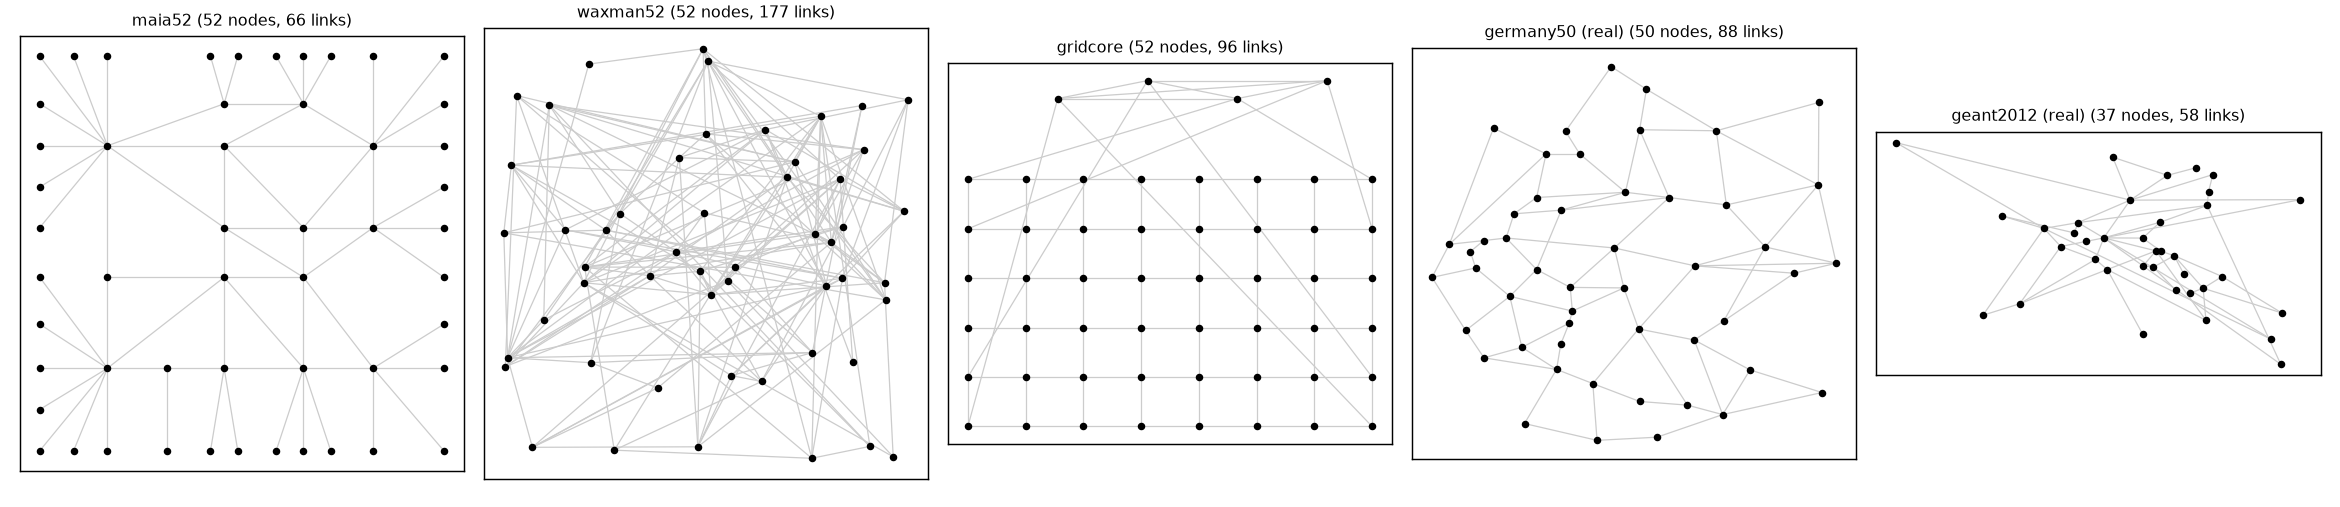
\includegraphics[width=\linewidth]{figures/fig11_topologies.png}
\caption{Evaluated 52-node instances: the original study topology (maia52)
and two synthetic instances (waxman52, gridcore). All share the same
17-flow demand profile and per-link capacity.}
\label{fig:topos}
\end{figure}

%=====================================================================
\section{Results}
\label{sec:results}

\subsection{Optimality Certification at Nominal Load}
\label{sec:cert}
At nominal load on maia52, the exact pool formulation ILP-P certifies the
pool optimum $\FO=\PoolOptFO$; ACO$+$GA attains it in every replication
(mean $\GaFOmaia\pm\GaFOmaiaCI$), matching the certified optimum, while
ACO$+$DE reaches $\DeFOmaia\pm\DeFOmaiaCI$ and the Q-learning agent
$\QlFOmaia\pm\QlFOmaiaCI$ (Fig.~\ref{fig:cert}). Dijkstra, which does not
optimize \eqref{eq:fo}, scores $\DjFOmaia$. The optimality gap of the hybrid
with respect to its own search space is therefore \emph{zero} --- a property
heuristic papers assert and rarely demonstrate. Table~\ref{tab:fo} shows the
same comparison on all three topologies: with the augmented pool the hybrid
attains the certified optimum on every instance and replication, whereas the
un-augmented pool made the selector seed-dependent --- before augmentation,
ACO$+$GA reached a feasible assembly in only half of the replications on
the sparse maia52 instance (50\% feasibility at nominal load), because pool
diversity, not the selector, is the binding constraint of generate-and-select
designs. On the revised model, ILP-L
finds a feasible solution with minimum-maximum utilization
$Z=\IlpZmaia$; CSPF and the hybrid also remain feasible at nominal load, but
without a balancing objective their utilization profiles are worse
(Section~\ref{sec:sweep}).
Fig.~\ref{fig:conv} shows the convergence dynamics behind those scores,
together with the constructive-seeding ablation: without pool augmentation
(grey), the same selector starts $\approx$16 FO points lower and
occasionally stalls below the optimum, while the augmented hybrid reaches
the certified optimum by generation $\approx$20 in every seed and is
monotonically stable afterwards; on the denser instances the optimal
assembly is already present from the first generation --- the convergence
effort concentrates precisely where the certified bounds are tightest.

\begin{table}[!t]
\caption{Objective-function score at nominal load (20 seeds, mean $\pm$
95\% CI). Dijkstra and CSPF are deterministic.}
\label{tab:fo}
\centering
\begin{tabular}{@{}lrrrrr@{}}
\toprule
Topology & Dijkstra & CSPF & Q-learn & ACO+DE & ACO+GA\\
\midrule
maia52 & 120 & 132 & 130$\pm$1 & 132$\pm$0 & 132$\pm$0\\
waxman52 & 132 & 132 & 132$\pm$0 & 132$\pm$0 & 132$\pm$0\\
gridcore & 130 & 132 & 132$\pm$0 & 132$\pm$0 & 132$\pm$0\\
germany50 & 128 & 132 & 132$\pm$1 & 132$\pm$0 & 132$\pm$0\\
geant2012 & 128 & 130 & 130$\pm$0 & 130$\pm$0 & 132$\pm$0\\
\bottomrule
\end{tabular}

\end{table}

\begin{figure}[!t]
\centering
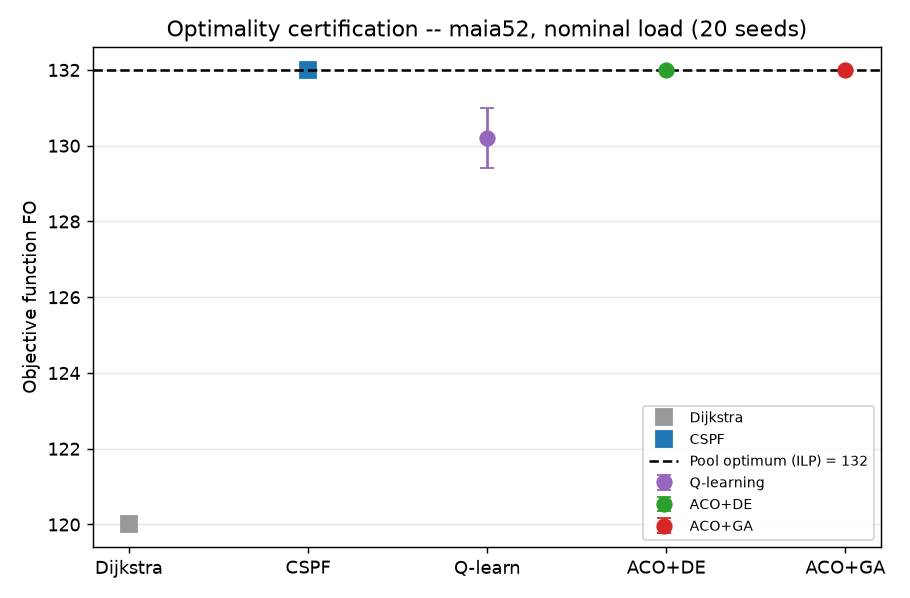
\includegraphics[width=\linewidth]{figures/fig8_optimality.png}
\caption{Objective-function scores at nominal load (maia52, 20 seeds, mean
$\pm$ 95\% CI). The dashed line is the exact pool optimum certified by
ILP-P; ACO$+$GA attains it in every replication.}
\label{fig:cert}
\end{figure}

\begin{figure}[!t]
\centering
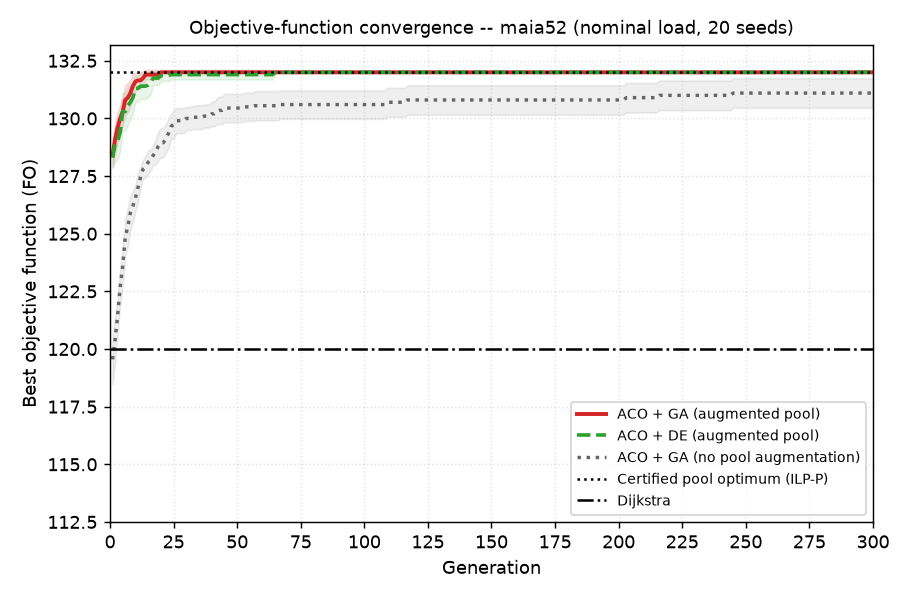
\includegraphics[width=\linewidth]{figures/fig2_convergence.png}
\caption{Objective-function convergence on maia52 at nominal load:
best-so-far FO per generation, mean $\pm$ 95\% CI over 20 seeds. The
pool-augmented hybrid reaches the certified optimum ($\FO=132$) by
generation $\approx$20 in every seed and never falls back below it; without
pool augmentation (grey), the same selector starts $\approx$16 FO points
lower and occasionally stalls below the optimum.}
\label{fig:conv}
\end{figure}

\subsection{Load Sweep: Exact Bottleneck Certification under Stress}
\label{sec:sweep}
The central exact-model result is the \emph{bottleneck lower bound}. At
$f=1.25$ on maia52, ILP-L certifies $Z^{*}=\IlpZmaiaHigh$: under hard
constraints, \emph{no} assignment of the 22 flows to any paths in $G$ can
keep every link below \IlpZmaiaHighPct\% utilization --- the instance is
provably at its limit, and
the certified bound quantifies exactly how tight. At $f=1.5$ the certified
bound reaches $Z^{*}=\IlpZmaiaMax$: some link must operate at full capacity under
every possible routing. On the denser waxman52 and the hierarchical
gridcore, the certified bound stays at $Z^{*}=0.872$ through the whole sweep
--- the exact model certifies that a $13\%$ headroom remains even at
$1.5\times$ load, information no heuristic can produce. Exact solves take
seconds (Table~\ref{tab:time}), making such certificates practical at this
scale.

Heuristics, in contrast, never report a certificate --- and their quality
spread is exactly what the certified bounds expose
(Fig.~\ref{fig:viol}, Table~\ref{tab:viol}). Dijkstra, oblivious to
capacity, inflicts $\DjViolHigh$ SLA violations at $f=1.25$ and
$\DjViolMax$ at $f=1.5$ on maia52, reaching \DjMaxUtil$\times$ link
capacity; CSPF remains violation-free up to $f=1.25$ but strands
\CspfViolMax\ overloaded links at $f=1.5$, whereas the pool-augmented
hybrid stays violation-free through the whole sweep and the un-augmented
Q-learning agent violates its budgets in every stressed load
(\QlViolHigh--\QlViolMax). The same ordering holds on the synthetic
topologies, where only Dijkstra violates (one to three overloaded links at
$f\ge1.25$). In operationally meaningful terms: \emph{the exact model tells
the operator how much headroom the network provably has; the hybrid keeps
the SLA intact whenever the pool permits; the learning-based agent provides
no such guarantee exactly when the network is tight}.

\begin{table}[!t]
\caption{SLA violations (overloaded links $+$ delay-violating flows) on
maia52: deterministic methods as counts, stochastic as mean $\pm$ 95\% CI
over 20 seeds.}
\label{tab:viol}
\centering
\begin{tabular}{@{}lrrrrr@{}}
\toprule
Load & Dijkstra & CSPF & Q-learn & ACO+DE & ACO+GA\\
\midrule
1.0$\times$ & 6+0 & 0+0 & 0.9$\pm$0.4 & 0.0$\pm$0.0 & 0.0$\pm$0.0\\
1.25$\times$ & 6+0 & 0+0 & 1.8$\pm$0.7 & 0.2$\pm$0.2 & 0.0$\pm$0.0\\
1.5$\times$ & 9+0 & 4+0 & 1.9$\pm$0.5 & 1.9$\pm$0.4 & 1.1$\pm$0.4\\
\bottomrule
\end{tabular}

\end{table}

\begin{figure}[!t]
\centering
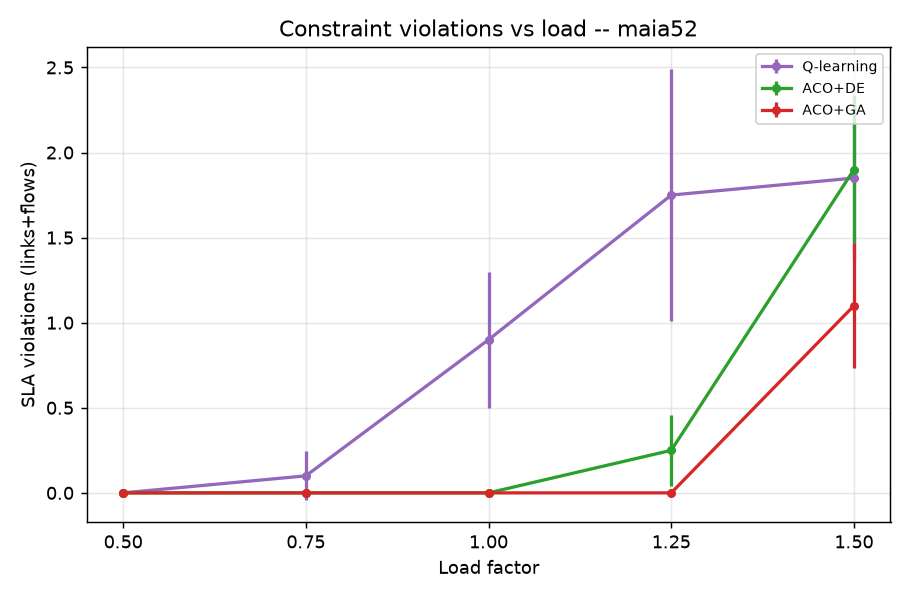
\includegraphics[width=\linewidth]{figures/fig6_violations_maia52.png}
\caption{SLA violations (overloaded links $+$ delay-violating flows) versus
load factor on maia52 (mean $\pm$ 95\% CI over 20 seeds). The pool-augmented
hybrid stays violation-free; shortest-path routing degrades first and the
Q-learning agent provides no feasibility guarantee.}
\label{fig:viol}
\end{figure}

\subsection{Load Balancing Quality}
Fig.~\ref{fig:maxutil} reports maximum link utilization on maia52. At
nominal load the exact min--max optimum is $Z=\IlpZmaia$; CSPF and the
hybrid remain near the capacity limit ($Z\approx 1.0$) but above the exact
value, and Dijkstra exceeds capacity entirely ($Z\approx\DjMaxUtil$). As
load grows past the feasibility frontier, utilization-based comparison
ceases to be meaningful (all methods exceed capacity); the violation counts
of Section~\ref{sec:sweep} then carry the operational signal.

\begin{figure}[!t]
\centering
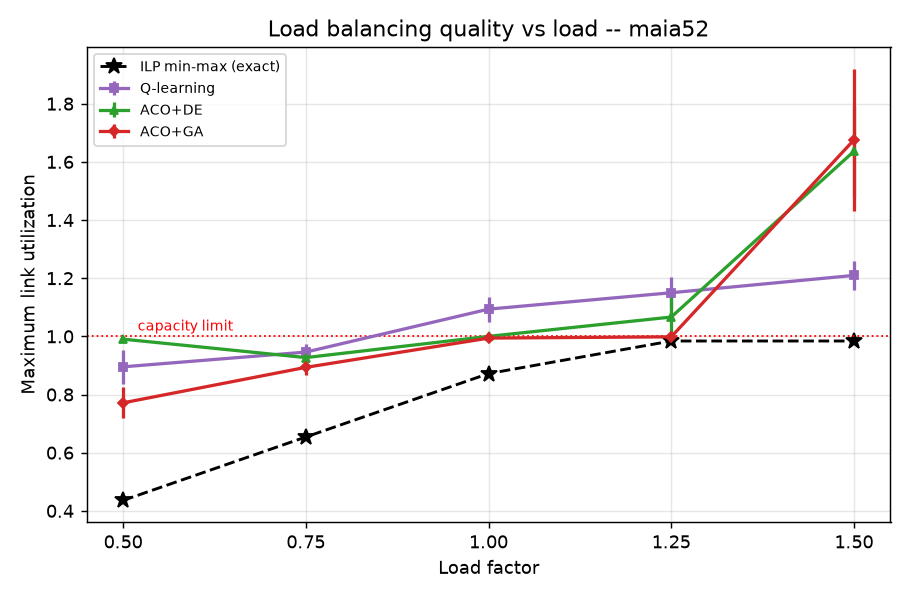
\includegraphics[width=\linewidth]{figures/fig7_maxutil_maia52.png}
\caption{Maximum link utilization versus load (maia52). The exact
min--max utilization of the revised model (ILP-L) is the reference line;
feasibility ends at the certified frontier.}
\label{fig:maxutil}
\end{figure}

\subsection{Packet-Level QoS under Identical Conditions}
\label{sec:qos}
With identical queues, capacities and injection rates, the optimized routing
sustains \SimThrGain\ higher mean goodput than Dijkstra and reduces mean
end-to-end delay from \SimDelayDj\,ms to \SimDelayOpt\,ms, jitter from
\SimJitDj\,ms to \SimJitOpt\,ms and loss from \SimLossDj\% to \SimLossOpt\%
(Fig.~\ref{fig:mininet}). The packet-level simulator is deterministic given
the routing and the constant-rate injection schedule (no stochastic
elements), so single-realization values are reported; all sampling
variability in this paper lives in the route-computation layer, where it is
replicated and tested (Section~\ref{sec:sweep}). The controlled simulation
reproduces the \emph{direction} of the emulated testbed results of the
original study with moderate magnitudes; Section~\ref{sec:bench} explains
why the bench magnitudes are larger. Notably, the certified min--max
routing (ILP-L) achieves better packet-level QoS than the score-optimal
hybrid routes --- balancing and feasibility translate directly into
queueing behavior.

\begin{figure}[!t]
\centering
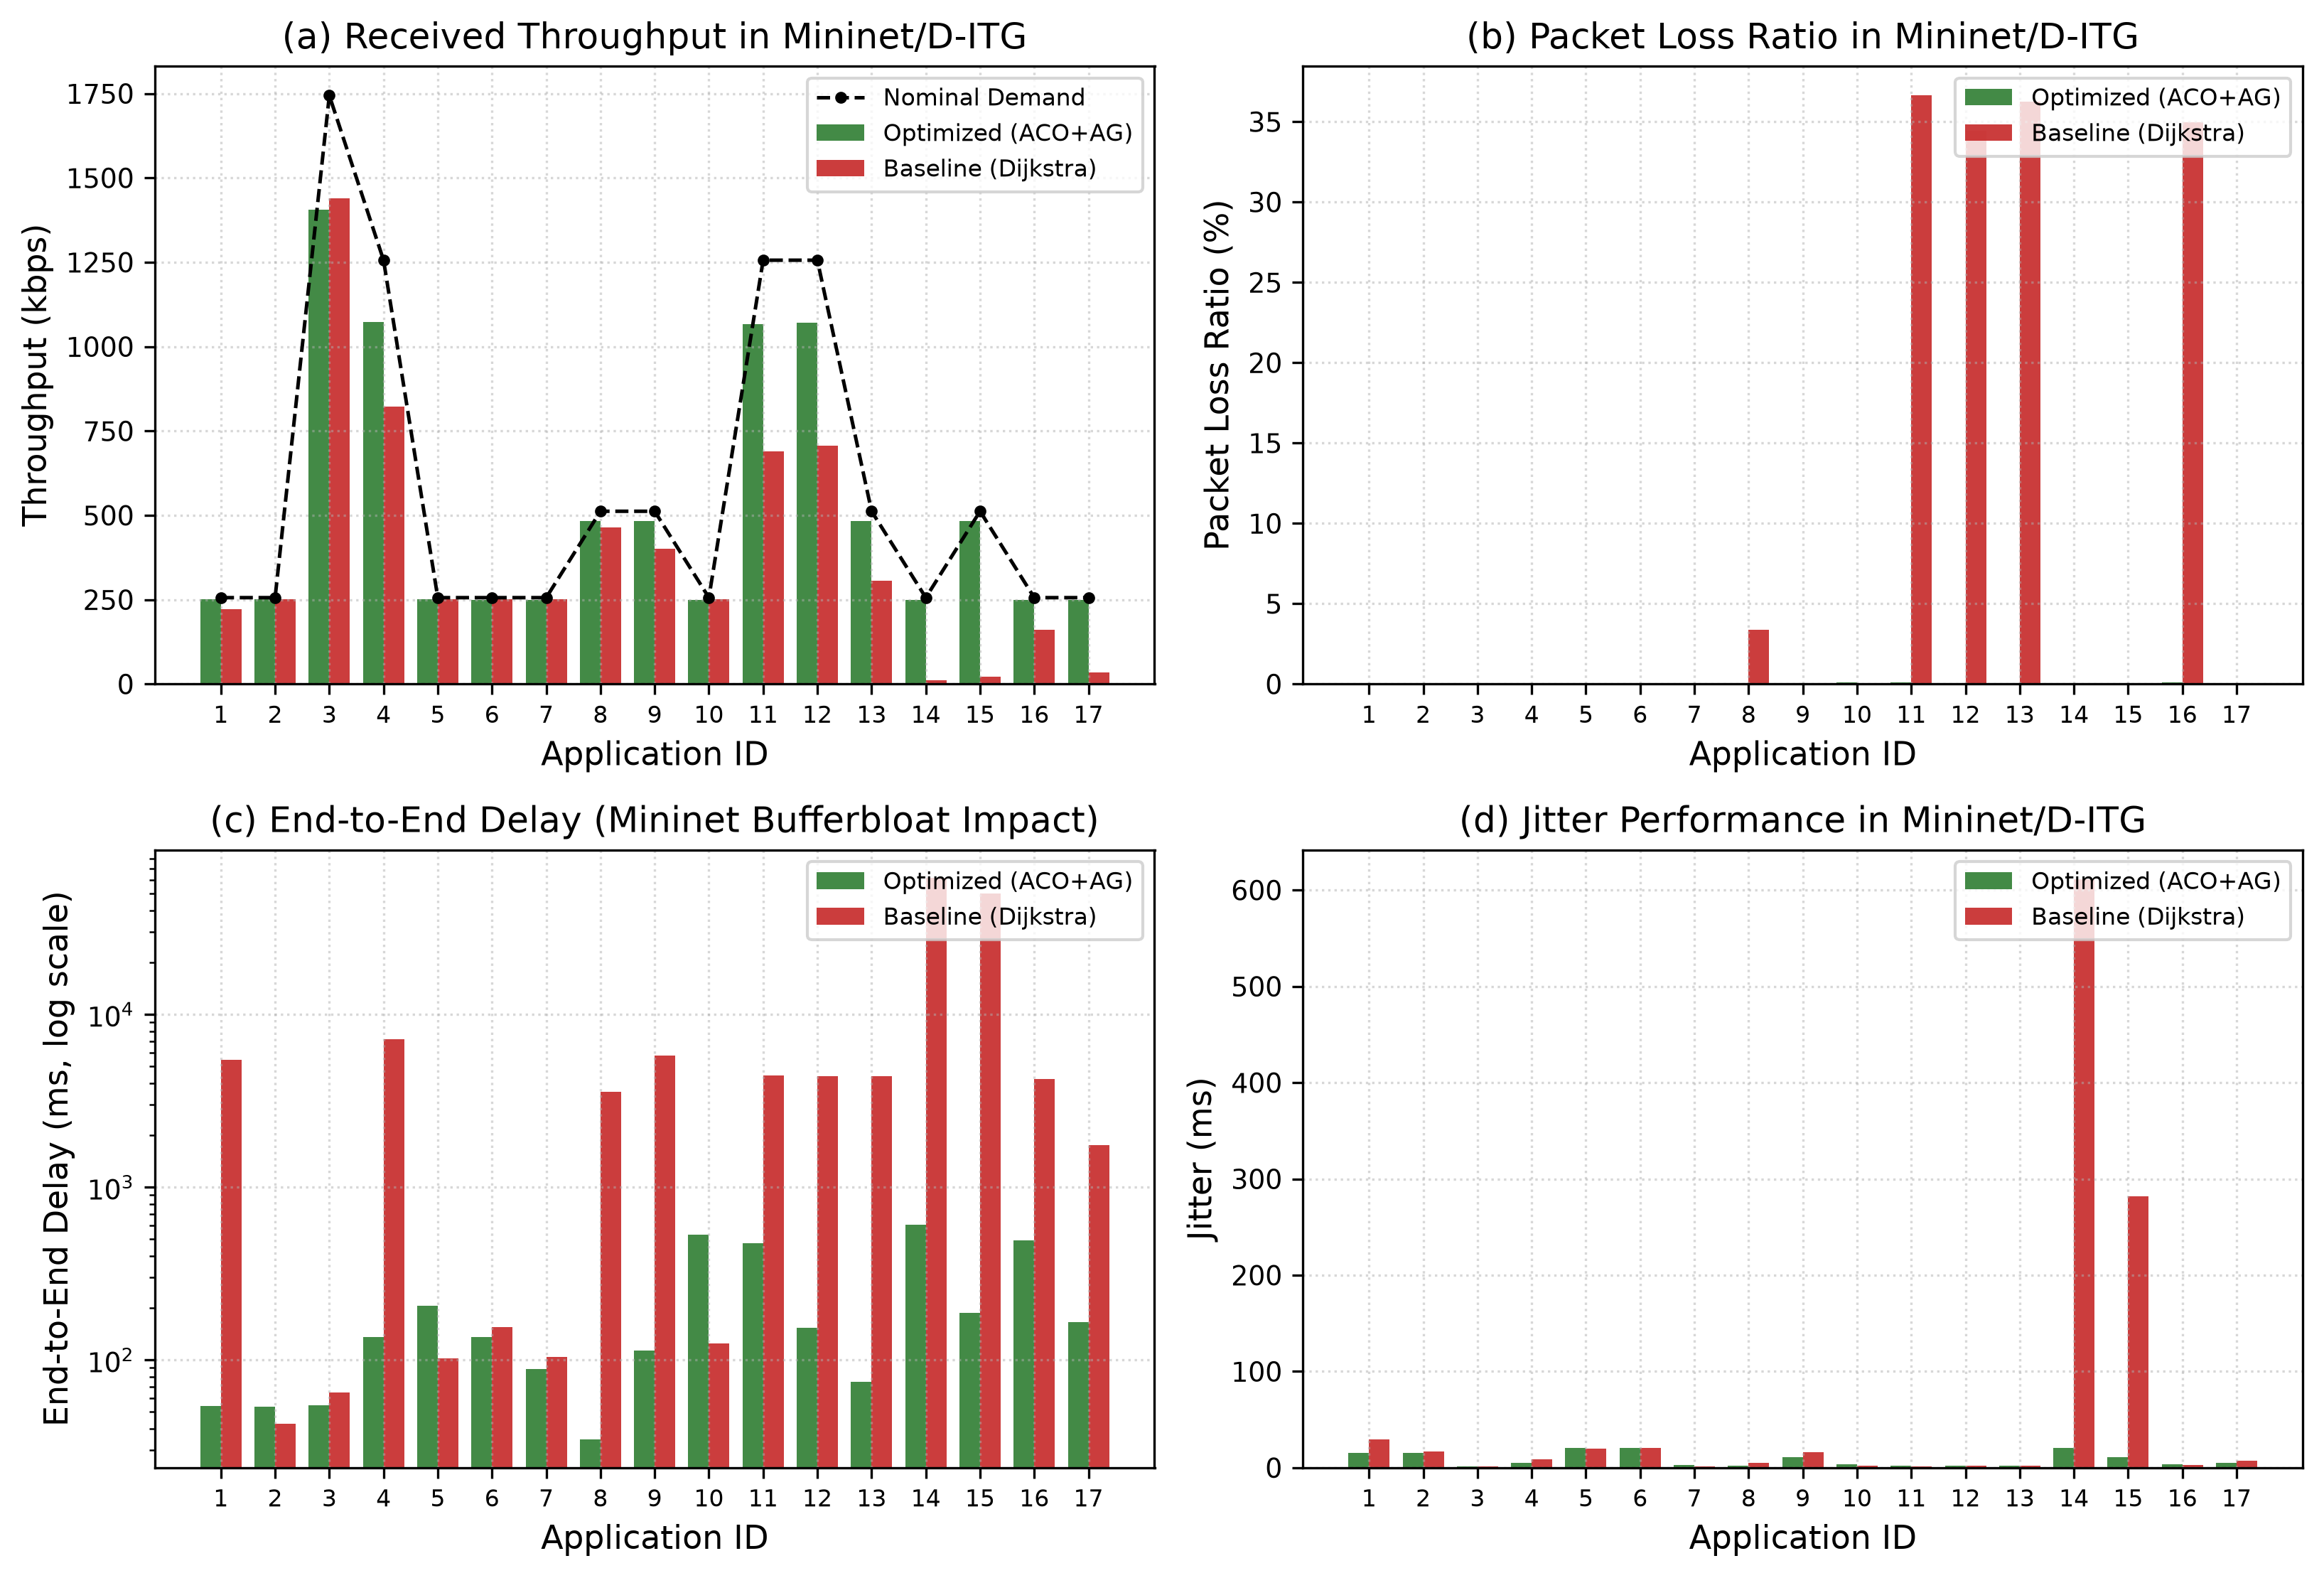
\includegraphics[width=\linewidth]{figures/fig3_mininet_results.png}
\caption{Emulated testbed (Mininet/Floodlight/D-ITG): per-application
throughput, loss, delay and jitter, optimized versus shortest-path routing
(original-study data). The direction of every effect matches the controlled
simulation; magnitudes differ (Section~\ref{sec:bench}).}
\label{fig:mininet}
\end{figure}

\subsection{Slice Isolation under Background Amplification}
\label{sec:slicesres}
Fig.~\ref{fig:slices} shows URLLC-grade flows at nominal rate while the
eMBB/mMTC background is amplified by $1\times$--$4\times$. With optimized
routing URLLC keeps its 150\,ms budget up to $2\times$ background
(\UrllcDoptOne\,ms at $1\times$, \UrllcDoptTwo\,ms at $2\times$) and its loss
stays below \UrllcLossOptTwo\% at $2\times$; with shortest-path routing the
same flows violate the budget at \emph{every} level
(\UrllcDdjOne\,ms at $1\times$) and lose up to \UrllcLossDjFour\% of packets at
$4\times$. The constraint structure of the optimizer --- aggregate
cross-slice capacity and per-slice delay budgets --- delivers measurable
logical isolation without any physical partitioning of the network.

\begin{figure*}[!t]
\centering
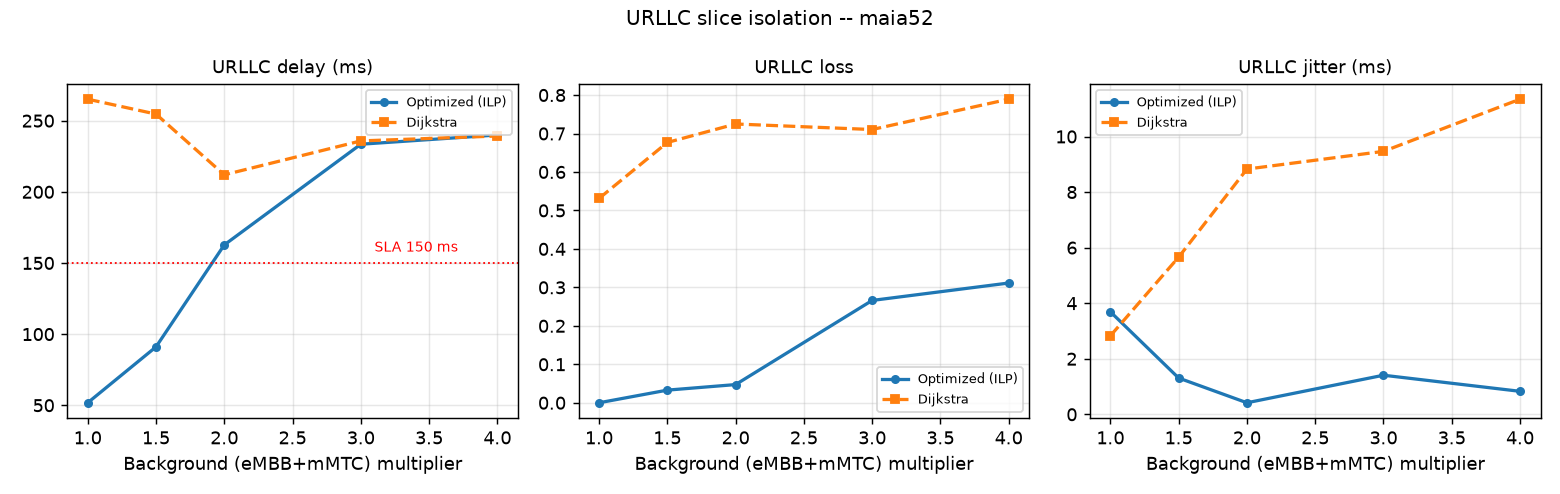
\includegraphics[width=0.92\textwidth]{figures/fig10_slice_isolation.png}
\caption{URLLC-grade flows (voice, 150\,ms SLA) under growing eMBB/mMTC
background amplification, optimized versus shortest-path routing. Optimized
routing preserves the SLA up to $2\times$ background; shortest-path routing
violates it at every level.}
\label{fig:slices}
\end{figure*}

\subsection{Measured SRv6 State Reduction}
\label{sec:srv6res}
Table~\ref{tab:srv6} and Fig.~\ref{fig:srv6} report the measured data-plane
state. Encoding the same optimized paths as SRv6 segment lists requires
exactly one rule per flow at its headend (\SrvSrRules\ rules for 17 flows)
and \emph{zero} per-flow state at transit nodes, against
\SrvOfMaia--\SrvOfGrid\ per-flow OpenFlow rules distributed over transit
switches on the three topologies --- measured reductions of \SrvRedMaia$\times$
(maia52), \SrvRedWax$\times$ (waxman52) and \SrvRedGrid$\times$ (gridcore).
The longest segment list is \MaxSLAll\ SIDs (gridcore), yielding a maximum
encapsulation overhead of \MaxSrhBytes\ bytes per packet --- within the
practical SRH budget; denser graphs produce shorter lists (mean
\MeanSLWax\ SIDs on waxman52). The reduction is structural: it holds for
every routing philosophy we measured (Dijkstra, CSPF and the optimizer),
because it moves the path state from the network into the packet.

\begin{figure}[!t]
\centering
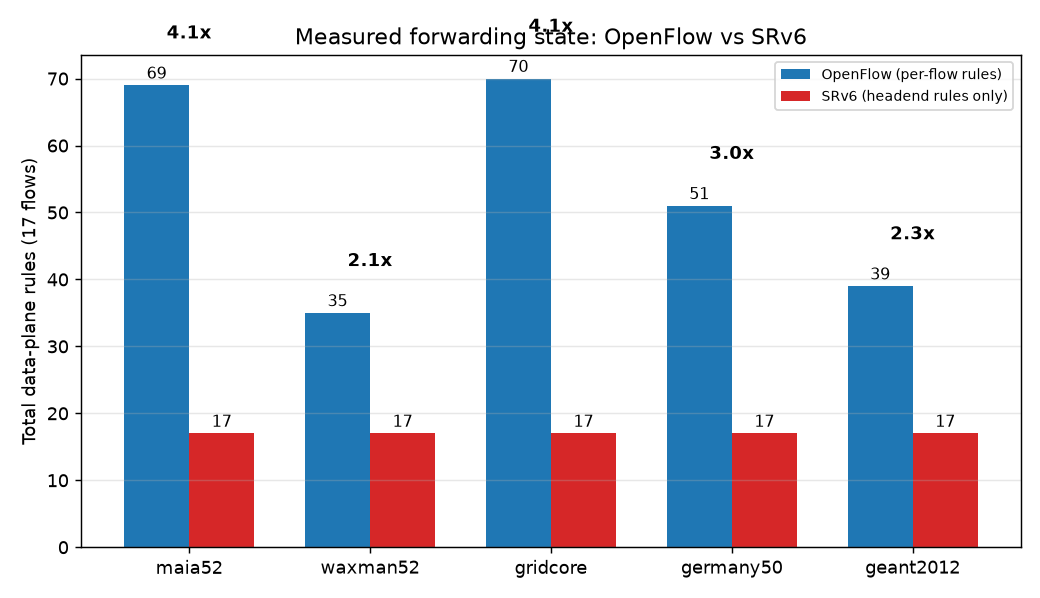
\includegraphics[width=\linewidth]{figures/fig9_srv6_state.png}
\caption{Measured forwarding state for the same 17-flow routing under
per-flow OpenFlow programming versus SRv6 headend-only programming.}
\label{fig:srv6}
\end{figure}

\begin{table}[!t]
\caption{Measured data-plane state (CSPF routing, 17 flows).}
\label{tab:srv6}
\centering
\begin{tabular}{@{}lrrrrr@{}}
\toprule
Topology & OF rules & OF max/node & SRv6 rules & Max SIDs & Reduction\\
\midrule
maia52 & 69 & 9 & 17 & 6 & 4.1$\times$\\
waxman52 & 35 & 4 & 17 & 4 & 2.1$\times$\\
gridcore & 70 & 4 & 17 & 10 & 4.1$\times$\\
germany50 & 51 & 5 & 17 & 6 & 3.0$\times$\\
geant2012 & 39 & 6 & 17 & 8 & 2.3$\times$\\
\bottomrule
\end{tabular}

\end{table}

\subsection{Learning-Based Baseline under the Same Protocol}
\label{sec:qlb}
The tabular Q-learning agent reaches $\QlFOmaia\pm\QlFOmaiaCI$ at nominal
load on maia52 --- near the certified optimum --- but its feasibility is
instance- and seed-sensitive: on the sparse maia52 it assembles a
violation-free route set in only \QlFeasNominal\% of replications at
nominal load, and under stress it inflicts $\QlViolHigh$ violations at
$f=1.25$ versus $\GaViolHigh$ for ACO$+$GA (Wilcoxon $p=\QlVsGaP$), while
on the denser synthetic instances it matches the certified optimum
everywhere. Its per-scenario training ($\QlTime$\,s) is spent again
at every new traffic epoch, whereas the metaheuristic recomputes from the
instantaneous state ($\GaTime$\,s). This measured pattern supports the
DRL-oriented argument at the heart of the learning-based routing debate:
learning-based routers can match deterministic optimizers on well-provisioned
regimes, but offer no constraint certificate, degrade off their training
distribution, and re-pay sampling costs per scenario
\cite{xu2018experience,stampa2017drl,almasan2022drl}. We therefore position
deterministic, constraint-explicit optimization as the decision core, with
learning as an upstream predictor --- not a replacement.

\subsection{Runtime}
All methods are fast enough for offline TE epochs (Table~\ref{tab:time}):
the exact pool ILP solves in $\PoolTime$\,s, the exact link ILP in
$\IlpTime$\,s, one hybrid run in $\GaTime$\,s, and Q-learning in
$\QlTime$\,s per scenario on a desktop-class CPU --- i.e., optimization
cost is not the operational bottleneck at this scale; certification value is
what distinguishes the methods.

\begin{table}[!t]
\caption{Median wall-clock runtime per complete routing decision (s).}
\label{tab:time}
\centering
\begin{tabular}{@{}lrr@{}}
\toprule
Method & Median runtime (s) & Model\\
\midrule
Dijkstra & 0.0 & deterministic\\
CSPF & 0.0 & deterministic\\
ACO+GA & 6.8 & stochastic\\
ACO+DE & 5.1 & stochastic\\
Q-learning & 0.2 & learning\\
ILP-P (pool) & 0.1 & exact\\
ILP-L (MCF) & 0.6 & exact\\
\bottomrule
\end{tabular}

\end{table}

\subsection{Reconciling Simulation and Emulation}
\label{sec:bench}
The controlled simulation and the emulated testbed agree on the direction of
every effect but differ in magnitude: the bench reports ratios of $51\times$
(delay) and $510\times$ (loss) against shortest-path routing, while the
controlled simulation reports \SimDelayRatio$\times$ and \SimLossRatio$\times$.
The explanation is the baseline, not the optimizer: with per-flow
shortest-path routing, a 2\,Mbps bottleneck link carrying several nominal
flows develops a deep persistent queue (bufferbloat; measured 10.8\,s of
queuing delay on the bench). The magnitude of the improvement therefore
depends primarily on queue sizing and queue management of the baseline
deployment --- a configuration artifact --- rather than on the optimizer
itself. We report the controlled simulation with fixed, modest buffers
(80 packets) as the reproducible reference, and the bench as qualitative
confirmation; we explicitly discourage quoting cross-configuration ratios
without stating the queue configuration.

%=====================================================================
\section{Threats to Validity and Limitations}
\label{sec:limits}
\textbf{Scale.} All instances have 52 nodes and 17 flows; the feasibility
frontier and the hybrid's advantage are demonstrated at this scale with
statistical replication, not at backbone scale. The ILP formulations scale
with $|E|\,L$ binaries and were solved in seconds here; larger instances
would need decomposition or column generation.
\textbf{Traffic model.} Constant-rate UDP-style injection abstracts away TCP
dynamics; TCP workloads with congestion control may shift the violation
frontier and are left for future work. The bench evidence (D-ITG) carries
the same abstraction.
\textbf{Pool reuse.} Candidate pools are generated at nominal load and
reused across the sweep; a load-adaptive pool could shift the frontier
slightly, although pool diversity is topology-driven.
\textbf{Objective weights.} The scoring model retains arbitrary weights by
design (continuity with the original formulation); all feasibility and
balancing conclusions are drawn from the revised model, which is
weight-free.
\textbf{Static demands.} The model optimizes a snapshot; reactive
re-optimization under churn and interaction with admission control are open
engineering problems.

%=====================================================================
\section{Conclusion}
\label{sec:conc}
We reformulated QoS-aware traffic engineering for SDN with hard capacity and
delay constraints and an explicit min--max balancing objective, and we closed
the methodological loop between heuristics and exactness: a two-stage hybrid
(ACO pool $+$ GA/DE selection) is certified against exact ILP solutions on
three topologies, five loads and twenty replications. The hybrid attains the
certified optimum of its search space at nominal load, minimizes SLA damage
in regimes certified infeasible, and outperforms both greedy and
learning-based baselines where it matters --- under stress. Mapping the
optimized paths to SRv6 cuts measured forwarding state by $2$--$4\times$ and
removes per-flow state from transit switches, and the constraint structure
delivers measurable URLLC isolation under background amplification without
physical sharding. The result is a practical, auditable and certifiable
traffic-engineering core for SDN controllers: deterministic enough for
mission-critical audit, exact where exactness is affordable, and heuristic
where scale demands it.

\section*{Reproducibility}
All experiments are produced by fixed-seed scripts (topology generation,
ACO pools, metaheuristics, Q-learning baseline, exact ILP models,
packet-level simulation, statistics and figures) released with this paper;
every number in the text is injected from the generated results files.

%=====================================================================
\begin{thebibliography}{30}

\bibitem{mckeown2008} N. McKeown \emph{et al.}, ``OpenFlow: Enabling
innovation in campus networks,'' \emph{ACM SIGCOMM Computer Communication
Review}, vol. 38, no. 2, pp. 69--74, 2008.

\bibitem{kim2013} H. Kim and N. Feamster, ``Improving network management with
software defined networking,'' \emph{IEEE Communications Magazine}, vol. 51,
no. 2, pp. 114--119, 2013.

\bibitem{hu2014} F. Hu, Q. Hao, and M. Bao, ``A survey on software-defined
network and OpenFlow: From concept to implementation,'' \emph{IEEE
Communications Surveys \& Tutorials}, vol. 16, no. 4, pp. 2181--2206, 2014.

\bibitem{bosshart2014} P. Bosshart \emph{et al.}, ``P4: Programming
protocol-independent packet processors,'' \emph{ACM SIGCOMM Computer
Communication Review}, vol. 44, no. 3, pp. 87--95, 2014.

\bibitem{dorigo2004} M. Dorigo and T. St\"utzle, \emph{Ant Colony
Optimization}. MIT Press, 2004.

\bibitem{waxman1988} B. M. Waxman, ``Routing of multipoint connections,''
\emph{IEEE Journal on Selected Areas in Communications}, vol. 6, no. 9,
pp. 1617--1622, 1988.

\bibitem{xu2018experience} H. Xu, Z. Li, L. Zhou, Z. Li, K. Wang, and Y.
Guo, ``Experience-driven networking: A deep reinforcement learning based
approach,'' in \emph{Proc. IEEE INFOCOM}, 2018, pp. 1871--1879.

\bibitem{stampa2017drl} A. Stampa, M. Arias, D. S\'anchez-Charles, P.
Barlet-Ros, and A. Cabellos-Aparicio, ``A deep-reinforcement learning
approach for software-defined networking routing optimization,'' arXiv
preprint arXiv:1709.07080, 2017.

\bibitem{almasan2022drl} P. Almasan, J. Su\'arez-Varela, A. Badia-Samper, P.
Barlet-Ros, and A. Cabellos-Aparicio, ``Towards deep reinforcement learning
for traffic engineering in SDN,'' \emph{Computer Networks}, vol. 213, art.
109035, 2022.

\bibitem{rfc8402} C. Filsfils, S. Previdi, L. Ginsberg, B. Decraene, S.
Litkowski, and R. Shakir, ``Segment Routing Architecture,'' IETF RFC 8402,
Jul. 2018.

\bibitem{rfc8754} C. Filsfils, D. Dukes, S. Previdi, J. Leddy, S.
Matsushima, and D. Voyer, ``IPv6 Segment Routing Header (SRH),'' IETF RFC
8754, Mar. 2020.

\bibitem{rfc8986} C. Filsfils, P. Camarillo, J. Leddy, D. Voyer, B.
Bernier, and J. Linkova, ``Segment Routing over IPv6 (SRv6) Network
Programming,'' IETF RFC 8986, Feb. 2021.

\bibitem{rfc9256} C. Filsfils, K. Talaulikar, D. Voyer, A. Bogdanov, and P.
Mattes, ``Segment Routing Policy Architecture,'' IETF RFC 9256, Jul. 2022.

\bibitem{rfc4655} A. Farrel, J.-P. Vasseur, and J. Ash, ``A Path Computation
Element (PCE)-Based Architecture,'' IETF RFC 4655, Aug. 2006.

\bibitem{itu-m2083} ITU-R, ``IMT Vision --- Framework and overall objectives
of the future development of IMT for 2020 and beyond,'' Recommendation
ITU-R M.2083-0, Sep. 2015.

\bibitem{3gpp-ts23501} 3GPP, ``System architecture for the 5G System
(5GS),'' Technical Specification TS 23.501, Release 17, 2022.

\bibitem{lantz2010} B. Lantz, B. Heller, and N. McKeown, ``A network in a
laptop: Rapid prototyping for software-defined networks,'' in \emph{Proc.
ACM HotNets}, 2010.

\bibitem{botta2012} A. Botta, A. Dainotti, and A. Pescap\'e, ``On the
validation of D-ITG,'' Technical Report, University of Napoli Federico II,
2012.

\bibitem{watkins1992} C. J. C. H. Watkins and P. Dayan, ``Q-learning,''
\emph{Machine Learning}, vol. 8, pp. 279--292, 1992.

\bibitem{itu2017} International Telecommunication Union, ``ICT facts and
figures 2017,'' Geneva, 2017.

\end{thebibliography}

\end{document}